\documentclass[a4paper,14pt]{extarticle}

\usepackage[utf8x]{inputenc}
\usepackage[T1,T2A]{fontenc}
\usepackage[russian]{babel}
\usepackage{hyperref}
\usepackage{indentfirst}
\usepackage{here}
\usepackage{array}
\usepackage{graphicx}
\usepackage{caption}
\usepackage{subcaption}
\usepackage{chngcntr}
\usepackage{amsmath}
\usepackage{amssymb}
\usepackage{pgfplots}
\usepackage{pgfplotstable}
\usepackage[left=2cm,right=2cm,top=2cm,bottom=2cm,bindingoffset=0cm]{geometry}
\usepackage{multicol}
\usepackage{askmaps}
\usepackage{titlesec}
\usepackage{listings}
\usepackage{color}
\usepackage{courier}

\definecolor{green}{rgb}{0,0.6,0}
\definecolor{gray}{rgb}{0.5,0.5,0.5}
\definecolor{purple}{rgb}{0.58,0,0.82}

\lstset{
	language=Verilog,
	backgroundcolor=\color{white},   
	basicstyle=\small\ttfamily,
	commentstyle=\color{green},
	keywordstyle=\color{blue},	
	numberstyle=\tiny\color{gray},
	stringstyle=\color{purple},
	breakatwhitespace=false,
	breaklines=true,
	captionpos=b,
	keepspaces=true,
	numbers=left,
	numbersep=5pt,
	showspaces=false,
	showstringspaces=false,
	showtabs=false,
	tabsize=4,
	frame=single,
	inputpath={../quartus/},
	literate={~} {$\sim$}{1}
}

\renewcommand{\le}{\ensuremath{\leqslant}}
\renewcommand{\leq}{\ensuremath{\leqslant}}
\renewcommand{\ge}{\ensuremath{\geqslant}}
\renewcommand{\geq}{\ensuremath{\geqslant}}
\renewcommand{\epsilon}{\ensuremath{\varepsilon}}
\renewcommand{\phi}{\ensuremath{\varphi}}
\renewcommand{\thefigure}{\arabic{figure}} 	
\renewcommand*\not[1]{\overline{#1}}

\titleformat*{\section}{\large\bfseries} 
\titleformat*{\subsection}{\normalsize\bfseries} 
\titleformat*{\subsubsection}{\normalsize\bfseries} 
\titleformat*{\paragraph}{\normalsize\bfseries} 
\titleformat*{\subparagraph}{\normalsize\bfseries} 

\counterwithin{figure}{section}
\counterwithin{equation}{section}
\counterwithin{table}{section}
\newcommand{\sign}[1][5cm]{\makebox[#1]{\hrulefill}}
\graphicspath{{../pics/}}
\captionsetup{justification=centering,margin=1cm}
\def\arraystretch{1.3}
\setlength\parindent{5ex}
\titlelabel{\thetitle.\quad}

\begin{document}

\begin{titlepage}
\begin{center}
	Санкт-Петербургский Политехнический Университет Петра Великого\\[0.3cm]
	Институт компьютерных наук и технологий \\[0.3cm]
	Кафедра компьютерных систем и программных технологий\\[4cm]
	
	\textbf{ОТЧЕТ}\\ 
	\textbf{по лабораторной работе}\\[0.5cm]
	\textbf{SystemVerilog №4}\\[0.1cm]
	Автоматизация проектирования\\ дискретных устройств\\[4.0cm]
\end{center}

\begin{flushright}
	\begin{minipage}{0.45\textwidth}
		\textbf{Работу выполнил студент}\\[3mm]
		группа 33501/4 \hspace*{9mm} Дьячков В.В.\\[5mm]
		\textbf{Преподаватель}\\[5mm]
		\sign[1.5cm] \hspace*{1mm} к.т.н., доц. Филиппов А.С. \\[5mm]
	\end{minipage}
\end{flushright}

\vfill

\begin{center}
	Санкт-Петербург\\
	\the\year
\end{center}
\end{titlepage}

\addtocounter{page}{1}
\counterwithin{lstlisting}{section}

\tableofcontents
\newpage
\lstlistoflistings
\listoffigures
\newpage

\section{Задание}

\begin{itemize}
	\item На языке Verilog на структурном уровне (с использованием только примитивов) создать иерархическое описание $3$-разрядного полного (с входом и выходом переноса) сумматора с последовательным переносом (переключатели задают двоичные коды данных; кнопка -- входной перенос; светодиоды отображают сумму и выходной перенос):
		\begin{itemize}
			\item Модуль -- \code{sum}; файл \code{sum.v}; проект в Quartus -- \code{sum};
			\item Рабочая папка -- \code{labs_6};
			\item Стандарты и номера выводов СБИС для платы \code{miniDiLaB_CIV} задать с помощью атрибутов.
		\end{itemize}
	
	\item На языке Verilog создать описание тестов:
		\begin{itemize}
			\item Тест класса 1 -- входные данные без знака \code{tb1_sum.v} и со знаком \code{tb1_sums.v};
			\item Тест класса 2 с вычислением результата -- входные данные без знака \code{tb2_sum.v} и со знаком \code{tb2_sums.v} (должен обеспечить проверку всех возможных вариантов входных сигналов);
			\item Тест класса 2 с чтением файлов -- входные данные без знака\\ \code{tb2f_sum.v} и со знаком \code{tb2f_sums.v} (файлы с тестовыми воздействиями -- \code{input_sum.dat} и \code{input_sum.dat}, файлы с ожидаемыми результатами -- \code{exp_sum.dat} и \code{exp_sums.dat}).
		\end{itemize}
	
	\item Осуществить проверку модуля с использованием всех тестов.
	
	\item Реализовать проект на плате \code{miniDiLaB_CIV}.
\end{itemize}

\section{Описание устройства}

В листинге \ref{code:sum_1} приведено описание одноразрядного сумматора.
\lstinputlisting[caption=\code{sum_1.v}, label=code:sum_1]{sum_1.v}

В листинге \ref{code:sum} приведено описание $N$-разрядного сумматора на основе одноразрядного.
\lstinputlisting[caption=\code{sum.v}, label=code:sum]{sum.v}

\section{Описание тестов}
\label{sec:tests}

\subsection{Тест первого класса}

\subsubsection{Входные данные без знака}

В листинге \ref{code:test1} приведено описание теста первого класса для входных данных без знака.
\lstinputlisting[caption=\code{tb1_sum.v}, label=code:test1]{tb1_sum.v}

В листинге \ref{code:test1_results} приведен вывод результатов теста в консоль.
\begin{lstlisting}[caption=Результаты теста первого класса (без знака), label=code:test1_results, style=console]
run -all
# 		           time a b c_in sum c_out
#                    0  0  0  0  0  0
#                    5  0  0  1  1  0
#                   10  0  1  1  2  0
#                   15  0  1  0  1  0
#                   20  0  2  0  2  0
...
#                  615  7  5  0  4  1
#                  620  7  6  0  5  1
#                  625  7  6  1  6  1
#                  630  7  7  1  7  1
#                  635  7  7  0  6  1
#    Time: 640 ns  Iteration: 0  Instance: /tb1_sum
\end{lstlisting}

На рис. \ref{fig:test1_results} изображена временная диаграмма теста.
\begin{figure}[H]
	\begin{center}
		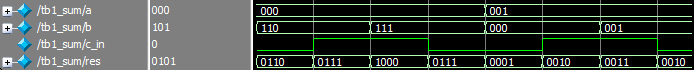
\includegraphics[width=1\textwidth]{test1_results}
		\caption{Результаты теста первого класса (без знака)}
		\label{fig:test1_results}
	\end{center}
\end{figure}

\subsubsection{Входные данные со знаком}

В листинге \ref{code:test1s} приведено описание теста первого класса для входных данных со знаком.
\lstinputlisting[caption=\code{tb1_sums.v}, label=code:test1s]{tb1_sums.v}

В листинге \ref{code:test1s_results} приведен вывод результатов теста в консоль.
\begin{lstlisting}[caption=Результаты теста первого класса (со знаком), label=code:test1s_results, style=console]
run -all
# 		            time a   b c_in sum c_out
#                    0   0   0  0   0  0
#                    5   0   0  1   1  0
#                   10   0   1  1   2  0
#                   15   0   1  0   1  0
#                   20   0   2  0   2  0
...
#                  615  -1  -3  0  -4  1
#                  620  -1  -2  0  -3  1
#                  625  -1  -2  1  -2  1
#                  630  -1  -1  1  -1  1
#                  635  -1  -1  0  -2  1
#    Time: 640 ns  Iteration: 0  Instance: /tb1_sums
\end{lstlisting}

На рис. \ref{fig:test1s_results} изображена временная диаграмма теста.
\begin{figure}[H]
	\begin{center}
		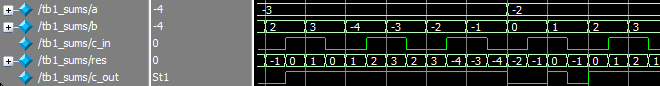
\includegraphics[width=1\textwidth]{test1s_results}
		\caption{Результаты теста первого класса (со знаком)}
		\label{fig:test1s_results}
	\end{center}
\end{figure}

\subsection{Тест второго класса с вычислением результата}

\subsubsection{Входные данные без знака}

В листинге \ref{code:test2} приведено описание теста второго класса с вычислением результата для входных данных без знака.
\lstinputlisting[caption=\code{tb2_sum.v}, label=code:test2]{tb2_sum.v}

В листинге \ref{code:test2_results} приведен вывод результатов теста в консоль.
\begin{lstlisting}[caption=Результаты теста второго класса с вычислением результата (без знака), label=code:test2_results, style=console]
run -all
# 		           time a b c_in sum c_out
#                    0  0  0  0  0  0
#                    5  0  0  1  1  0
#                   10  0  1  1  2  0
#                   15  0  1  0  1  0
#                   20  0  2  0  2  0
...
#                  615  7  5  0  4  1
#                  620  7  6  0  5  1
#                  625  7  6  1  6  1
#                  630  7  7  1  7  1
#                  635  7  7  0  6  1
# Testing complited
#    Time: 640 ns  Iteration: 0  Instance: /tb2_sum
\end{lstlisting}

На рис. \ref{fig:test2_results} изображена временная диаграмма теста.
\vspace{-0.5cm}
\begin{figure}[H]
	\begin{center}
		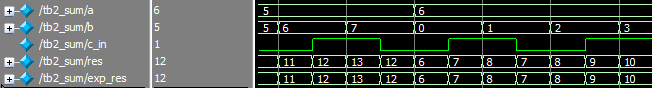
\includegraphics[width=0.95\textwidth]{test2_results}
		\caption{Результаты теста второго класса с вычислением результата (без знака)}
		\label{fig:test2_results}
	\end{center}
\end{figure}

В листинге \ref{code:test2_error} приведен вывод результатов теста в консоль при внесении ошибки в вычисление ожидаемого значения.	
\begin{lstlisting}[caption=Результаты ошибочного теста второго класса с вычислением результата (без знака), label=code:test2_error, style=console]
run -all
# 		 time a b c_in sum c_out
#                    0  0  0  0  0  0
# Expected  0, got  1.
# 
#                    5  0  0  1  1  0
# Expected  1, got  2.
...
#                  620  7  6  0  5  1
# Expected 13, got 14.
# 
#                  625  7  6  1  6  1
# Expected 14, got 15.
# 
#                  630  7  7  1  7  1
#                  635  7  7  0  6  1
# Testing complited
#    Time: 640 ns  Iteration: 0  Instance: /tb2_sum
\end{lstlisting}

\subsubsection{Входные данные со знаком}

В листинге \ref{code:test2s} приведено описание теста второго класса с вычислением результата для входных данных со знаком.
\lstinputlisting[caption=\code{tb2_sums.v}, label=code:test2s]{tb2_sums.v}

В листинге \ref{code:test2s_results} приведен вывод результатов теста в консоль.
\begin{lstlisting}[caption=Результаты теста второго класса с вычислением результата (со знаком), label=code:test2s_results, style=console]
run -all
# 		 time a b c_in sum c_out
#                    0   0   0  0   0  0
#                    5   0   0  1   1  0
#                   10   0   1  1   2  0
#                   15   0   1  0   1  0
#                   20   0   2  0   2  0
...
#                  615  -1  -3  0  -4  1
#                  620  -1  -2  0  -3  1
#                  625  -1  -2  1  -2  1
#                  630  -1  -1  1  -1  1
#                  635  -1  -1  0  -2  1
# Testing complited
#    Time: 640 ns  Iteration: 0  Instance: /tb2_sums
\end{lstlisting}

На рис. \ref{fig:test2s_results} изображена временная диаграмма теста.
\vspace{-0.5cm}
\begin{figure}[H]
	\begin{center}
		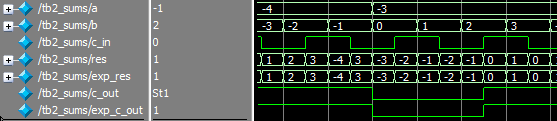
\includegraphics[width=0.9\textwidth]{test2s_results}
		\caption{Результаты теста второго класса с вычислением результата (со знаком)}
		\label{fig:test2s_results}
	\end{center}
\end{figure}

В листинге \ref{code:test2s_error} приведен вывод результатов теста в консоль при внесении ошибки в вычисление ожидаемого значения.	
\begin{lstlisting}[caption=Результаты ошибочного теста второго класса с вычислением результата (со знаком), label=code:test2s_error, style=console]
run -all
# 		           time a b c_in sum c_out
#                    0   0   0  0   0  0
# Expected (0, 0), got (0, 1).
# 
#                    5   0   0  1   1  0
# Expected (0, 1), got (0, 2).
...
#                  620  -1  -2  0  -3  1
# Expected (1,-3), got (1,-2).
# 
#                  625  -1  -2  1  -2  1
# Expected (1,-2), got (1,-1).
# 
#                  630  -1  -1  1  -1  1
#                  635  -1  -1  0  -2  1
# Testing complited
#    Time: 640 ns  Iteration: 0  Instance: /tb2_sums
\end{lstlisting}

\subsection{Тест второго класса с чтением файлов}

\subsubsection{Входные данные без знака}

В листинге \ref{code:test3} приведено описание теста второго класса с чтением файлов для входные данных без знака. В данном тесте на вход устройства из файла \code{input_sum.dat}, фрагмент которого приведен в листинге \ref{code:input}, подаются всевозможные значения, а ожидаемые считываются из файла \code{exp_sum.dat}, фрагмент которого приведен в листинге \ref{code:exp}.
\lstinputlisting[caption=\code{tb2f_sum.v}, label=code:test3]{tb2f_sum.v}

\newpage

\begin{multicols}{2}
	\lstinputlisting[caption=\code{input_sum.dat}, label=code:input, style=dat,linerange={1-5,123-128}]{input_sum.dat}	
	\lstinputlisting[caption=\code{exp_sum.dat}, label=code:exp, style=dat, linerange={1-5,123-128}]{exp_sum.dat}
\end{multicols}

В листинге \ref{code:test3_results} приведен вывод результатов теста в консоль.
\begin{lstlisting}[caption=Результаты теста второго класса с чтением файлов (без знака), label=code:test3_results, style=console]
run -all
# 		           time a b c_in sum c_out
#                    0  0  0  0  0  0
#                    5  0  0  1  1  0
#                   10  0  1  1  2  0
#                   15  0  1  0  1  0
#                   20  0  2  0  2  0
...
#                  615  7  5  0  4  1
#                  620  7  6  0  5  1
#                  625  7  6  1  6  1
#                  630  7  7  1  7  1
#                  635  7  7  0  6  1
# Testing complited
#    Time: 640 ns  Iteration: 0  Instance: /tb2f_sum
\end{lstlisting}

На рис. \ref{fig:test3_results} изображена временная диаграмма теста.
\begin{figure}[H]
	\begin{center}
		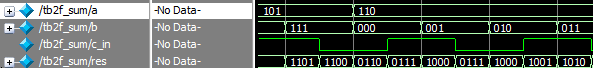
\includegraphics[width=0.9\textwidth]{test3_results}
		\caption{Результаты теста второго класса с чтением файлов (без знака)}
		\label{fig:test3_results}
	\end{center}
\end{figure}

В листинге \ref{code:test3_error} приведен вывод результатов теста в консоль при внесении ошибок в ожидаемые значения.
\newpage
\begin{lstlisting}[caption=Результаты ошибочного теста второго класса с чтением файлов, label=code:test3_error, style=console]
# 		          time a b c_in sum c_out
#                    0  0  0  0  0  0
# Expected  0, got  1.
# 
#                    5  0  0  1  1  0
# Expected  1, got  2.
# 
#                   10  0  1  1  2  0
#                   15  0  1  0  1  0
#                   20  0  2  0  2  0
# Expected  2, got  3.
...
# Expected 13, got 14.
# 
#                  625  7  6  1  6  1
# Expected 14, got 15.
# 
#                  630  7  7  1  7  1
# Expected 15, got 14.
# 
#                  635  7  7  0  6  1
# Testing complited
#    Time: 640 ns  Iteration: 0  Instance: /tb2f_sum
\end{lstlisting}

\subsubsection{Входные данные со знаком}

В листинге \ref{code:test3s} приведено описание теста второго класса с чтением файлов для входные данных со знаком. В данном тесте на вход устройства из файла \code{input_sums.dat}, фрагмент которого приведен в листинге \ref{code:inputs}, подаются всевозможные значения, а ожидаемые считываются из файла \code{exp_sums.dat}, фрагмент которого приведен в листинге \ref{code:exps}.
\lstinputlisting[caption=\code{tb2f_sums.v}, label=code:test3s]{tb2f_sums.v}

\begin{multicols}{2}
	\lstinputlisting[caption=\code{input_sums.dat}, label=code:inputs, style=dat,linerange={1-5,123-128}]{input_sums.dat}	
	\lstinputlisting[caption=\code{exp_sums.dat}, label=code:exps, style=dat, linerange={1-5,123-128}]{exp_sums.dat}
\end{multicols}

В листинге \ref{code:test3s_results} приведен вывод результатов теста в консоль.
\begin{lstlisting}[caption=Результаты теста второго класса с чтением файлов (без знака), label=code:test3s_results, style=console]
run -all
# 		           time  a  b c_in sum c_out
#                    0   0   0  0   0  0
#                    5   0   0  1   1  0
#                   10   0   1  1   2  0
#                   15   0   1  0   1  0
#                   20   0   2  0   2  0
...
#                  615  -1  -3  0  -4  1
#                  620  -1  -2  0  -3  1
#                  625  -1  -2  1  -2  1
#                  630  -1  -1  1  -1  1
#                  635  -1  -1  0  -2  1
# Testing complited
#    Time: 640 ns  Iteration: 0  Instance: /tb2f_sums
\end{lstlisting}

На рис. \ref{fig:test3s_results} изображена временная диаграмма теста.
\begin{figure}[H]
	\begin{center}
		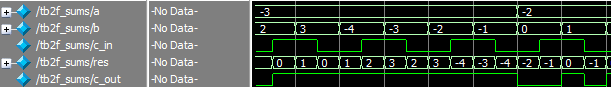
\includegraphics[width=1\textwidth]{test3s_results}
		\caption{Результаты теста второго класса с чтением файлов (со знаком)}
		\label{fig:test3s_results}
	\end{center}
\end{figure}

В листинге \ref{code:test3s_error} приведен вывод результатов теста в консоль при внесении ошибок в ожидаемые значения.
\begin{lstlisting}[caption=Результаты ошибочного теста второго класса с чтением файлов, label=code:test3s_error, style=console]
# 		           time  a  b c_in sum c_out
#                    0   0   0  0   0  0
# Expected   0, got  1.
# 
#                    5   0   0  1   1  0
# Expected   1, got  2.
...
#                  625  -1  -2  1  -2  1
# Expected  -2, got 15.
# 
#                  630  -1  -1  1  -1  1
# Expected  -1, got 14.
# 
#                  635  -1  -1  0  -2  1
# Testing complited
#    Time: 640 ns  Iteration: 0  Instance: /tb2f_sums
\end{lstlisting}

\newpage

\section{Тестирование на плате miniDiLaB\_CIV}

Для тестирования проекта на плате было создано Verilog описание с назначением выходов, приведенное в листинге  \ref{code:dilab}.
\lstinputlisting[caption=\code{dilab_sum.v}, label=code:dilab]{dilab_sum.v}

Результаты тестирования совпадают с ожидаемыми, следовательно, устройство работает верно.

\section{Выводы}

В ходе лабораторной работы на языке Verilog описан на структурном уровне (с использованием только примитивов) $3$-разрядный полный (с входом и выходом переноса) сумматор с последовательным переносом. Создано описание тестов первого и второго уровней, а также модуль для проверки работы на плате \code{miniDiLaB_CIV}. Тестирование разработанного устройства показало, что результаты совпадают с ожидаемыми и устройство работает верно.

\end{document}